\chapter{HDMI}\label{chap:chap3}

Este capítulo descreve o trabalho realizado para cumprir a primeira parte do projeto: obter uma conexão HDMI entre recetor e transmissor. São descritas as várias configurações das placas HDMI disponiveis e ainda as arquiteturas desenvolvidas e implementadas para cumprir esta parte do projeto. 

\section{\textit{Hardware} utilizado}

Tal como mencionado no sub-capítulo \ref{sec:HDMIinFPGA}, para receber os dados provenientes do cabo HDMI e fazer a sua selecção são utilizadas duas placas HDMI (TB-FMCH-HDMI2 RX E TB-FMCH-HDMI2 TX) que, através das suas entradas e saída FMC de alta velocidade, conseguem enviar para a FPGA os sinais de imagem e som. Nas imagens \ref{fig:rx} e \ref{fig:tx} é possivel visualizar o recetor (TB-FMCH-HDMI2 RX) e o transmissor (TB-FMCH-HDMI2 TX) HDMI utilizados neste projeto. Em conjunto, estas duas placas são designadas apenas por TB-FMCH-HDMI2. Estas mesmas placas são constituidas por conectores HDMI, de seguida o sinal é enviado para um recetor ou transmissor HDMI, ADV7612 no caso do recetor e ADV7511 no caso do transmissor. Finalmente os sinais provenientes do recetor/transmissor são enviados para uma FGPA embebida na placa (XC6SLX45-3FGG484C) que, consoante a sua configuração, envia pelos conectores FMC os sinais de audio e video.

As placas possuem ainda uma PROM (\textit{Programmable read-only memory}) XCF16PFSG48C de configuração reprogramável que permite armazenar o \textit{bitstream} que configura a FPGA embebida do modo que se pretende. É esta FPGA embebida que em cada placa (RX e TX) é responsável pela selecção e envio dos dados pretendidos para os conectores FMC (e posterior envio para a FPGA), e como tal é necessário que estejam configuradas para realizarem tais procedimentos. O recurso a estas memórias reconfiguraveis vem permitir uma fácil alteração da configuração da FPGA uma vez que, segundo \cite{R026}, estas memórias de leitura permitem não só armazenar os \textit{bitstreams} de configuração da FPGA, mas também reconfigurá-los, caso se pretenda, de uma forma fácil e eficiente.

\subsection{Configurações da FPGA} \label{subsec:HDMIconfig}

A FPGA \textit{Spartan-6} (XC6SLX45-3FGG484C) embebida nas placas tem 3 configurações disponiveis. Estas configurações variam não só no suporte que têm, que pode ser apenasde imagem mas também de imagem e audio, mas variam também no número de bits por imagem que estas podem ter. Nas secções seguintes serão brevemente expostas as configurações disponiveis e como se pode tirar partido das mesmas no projeto.


\subsubsection{Configuração por \textit{default}} \label{subsubsec:HDMIconfigdefault}

Esta configuração vem previamente escrita na memória PROM de fábrica e acaba por ser a mais simples de todas. Os dados enviados pelos conectores FMC são apenas referentes aos dados de imagem. As tabela \ref{table:HDMIdataRX} e \ref{table:HDMIdataTX} nas páginas \pageref{table:HDMIdataRX} e \pageref{table:HDMIdataTX} respectivamente identificam os pinos aos quais são atribuídas os sinais de dados de imagem HDMI tanto no recetor como no transmissor.

Esta configuração apenas transmite imagens RGB (\textit{Red Green Blue}) com 10 bits. Assim sendo, independetemente da formatação das imagens da fonte HDMI, o recetor ADV7612 presente na placa recetora HDMI converte a imagem para o formato RGB com 10 bits. Segundo \cite{R016}, 


A tabela \ref{table:HDMIdataDefaultdetail} apresentada na página \pageref{table:HDMIdataDefaultdetail} mostra com  mais detalhe as portas utilizadas tanto no transmissor como no recetor e ainda quais os \textit{bits} que representam em cada imagem. Esta tabela foi adaptada de \cite{R009} onde são apresentados os detalhes de todos os conectores FMC.

--> FALAR UM POUCO DO ADV7612 no sentido de explicar essa transformação??


\begin{table}[h!]
	\centering
	\begin{tabular}{|c|c|c|c|}
		\hline
		\textbf{PIN} & \textbf{FPGA -\textgreater FMC (RX)} & \textbf{FMC->FPGA (TX)} & \textbf{Descrição}       \\ \hline
		CLK0\_M2C\_P & RX\#O\_LLC                           & TX\#O\_DCLK                        & \textit{clock} dos pixeis         \\ \hline
		LA00\_P\_CC  & RX\#0\_VSYNC                         & TX\#0\_VSYNC                       & sincr. Vertical          \\ \hline
		LA01\_P\_CC  & RX\#0\_HSYNC                         & TX\#0\_HSYNC                       & sincr. Horizontal        \\ \hline
		LA02\_P      & RX\#0\_DE                            & TX\#0\_DE                          & sinal de dados ativos    \\ \hline
		LA03\_P      & RX\#0\_P0                            & TX\#0\_D0                          & Pixel de imagem B{[}0{]} \\ \hline
		LA04\_P      & RX\#0\_P1                            & TX\#0\_D1                          & Pixel de imagem B{[}1{]} \\ \hline
		LA05\_P      & RX\#0\_P2                            & TX\#0\_D2                          & Pixel de imagem B{[}2{]} \\ \hline
		LA06\_P      & RX\#0\_P3                            & TX\#0\_D3                          & Pixel de imagem B{[}3{]} \\ \hline
		LA07\_P      & RX\#0\_P4                            & TX\#0\_D4                          & Pixel de imagem B{[}4{]} \\ \hline
		LA08\_P      & RX\#0\_P5                            & TX\#0\_D5                          & Pixel de imagem B{[}5{]} \\ \hline
		LA09\_P      & RX\#0\_P6                            & TX\#0\_D6                          & Pixel de imagem B{[}6{]} \\ \hline
		LA10\_P      & RX\#0\_P7                            & TX\#0\_D7                          & Pixel de imagem B{[}7{]} \\ \hline
		LA11\_P      & RX\#0\_P8                            & TX\#0\_D8                          & Pixel de imagem B{[}8{]} \\ \hline
		LA12\_P      & RX\#0\_P9                            & TX\#0\_D9                          & Pixel de imagem B{[}9{]} \\ \hline
		LA13\_P      & RX\#0\_P10                           & TX\#0\_D10                         & Pixel de imagem G{[}0{]} \\ \hline
		LA14\_P      & RX\#0\_P11                           & TX\#0\_D11                         & Pixel de imagem G{[}1{]} \\ \hline
		LA15\_P      & RX\#0\_P12                           & TX\#0\_D12                         & Pixel de imagem G{[}2{]} \\ \hline
		LA16\_P      & RX\#0\_P13                           & TX\#0\_D13                         & Pixel de imagem G{[}3{]} \\ \hline
		LA17\_P\_CC  & RX\#0\_P14                           & TX\#0\_D14                         & Pixel de imagem G{[}4{]} \\ \hline
		LA18\_P\_CC  & RX\#0\_P15                           & TX\#0\_D15                         & Pixel de imagem G{[}5{]} \\ \hline
		LA19\_P      & RX\#0\_P16                           & TX\#0\_D16                         & Pixel de imagem G{[}6{]} \\ \hline
		LA20\_P      & RX\#0\_P17                           & TX\#0\_D17                         & Pixel de imagem G{[}7{]} \\ \hline
		LA21\_P      & RX\#0\_P18                           & TX\#0\_D18                         & Pixel de imagem G{[}8{]} \\ \hline
		LA22\_P      & RX\#0\_P19                           & TX\#0\_D19                         & Pixel de imagem G{[}9{]} \\ \hline
		LA23\_P      & RX\#0\_P20                           & TX\#0\_D20                         & Pixel de imagem R{[}0{]} \\ \hline
		LA24\_P      & RX\#0\_P21                           & TX\#0\_D21                         & Pixel de imagem R{[}1{]} \\ \hline
		LA25\_P      & RX\#0\_P22                           & TX\#0\_D22                         & Pixel de imagem R{[}2{]} \\ \hline
		LA26\_P      & RX\#0\_P23                           & TX\#0\_D23                         & Pixel de imagem R{[}3{]} \\ \hline
		LA27\_P      & RX\#0\_P24                           & TX\#0\_D24                         & Pixel de imagem R{[}4{]} \\ \hline
		LA28\_P      & RX\#0\_P25                           & TX\#0\_D25                         & Pixel de imagem R{[}5{]} \\ \hline
		LA29\_P      & RX\#0\_P26                           & TX\#0\_D26                         & Pixel de imagem R{[}6{]} \\ \hline
		LA30\_P      & RX\#0\_P27                           & TX\#0\_D27                         & Pixel de imagem R{[}7{]} \\ \hline
		LA31\_P      & RX\#0\_P28                           & TX\#0\_D28                         & Pixel de imagem R{[}8{]} \\ \hline
		LA32\_P      & RX\#0\_P29                           & TX\#0\_D29                         & Pixel de imagem R{[}9{]} \\ \hline
	\end{tabular}
	\caption{Localização dos pinos de dados utilizados em TB-FMCH-HDMI2 configurado por \textit{default}}
	\label{table:HDMIdataDefaultdetail}
\end{table}

É de notar ainda que esta configuração é capaz de suportar até dois canais (RX0 e TX0, RX1 e TX1), no entanto nesta tabela apenas são apresentados os dados correspondentes ao canal 0 pois apenas será necessário utilizar um canal neste projeto. 

Apesar de ser um configuração simples, uma vez que apenas são transmitidos sinais de imagem em formato RGB, é uma configuração que será utilizada numa fase inicial em algumas arquiteturas implementadas que serão descritas no subcapitulo \ref{subsec:HDMIarquiteturas}.

\subsubsection{1 canal e suporte de audio} \label {subsubsec:HDMIconfig+audio}

Esta configuração trata-se de uma configuração capaz de suportar não só imagens em formato YCbCr mas também RGB com 12 bits, como também suporta audio em formato $I^{2}$S. A configuração da imagem está dependente da fonte HDMI, e é transmitida pelas placas tal como é emitida pela fonte, por outras palavras, se a fonte HDMI transmitir uma imagem em formato RGB, é nesse formato que chega ao destino, no entanto se for transmitida uma imagem no formato YCbCr é nesse formato que chega ao seu destino.



\subsubsection{2 canais melhorado} \label{subsubsec:HDMIconfigMelhorado}

--> Falar como é que se reconfigurou as placas

\subsection{Configuração dos \textit{switches}}

\subsection{Arquiteturas Desenvolvidas} \label{subsec:HDMIarquiteturas}

\subsubsection{Transmissão de uma imagem gerada na FPGA}

		\begin{figure}[h!]
	\begin{center}
		\leavevmode
		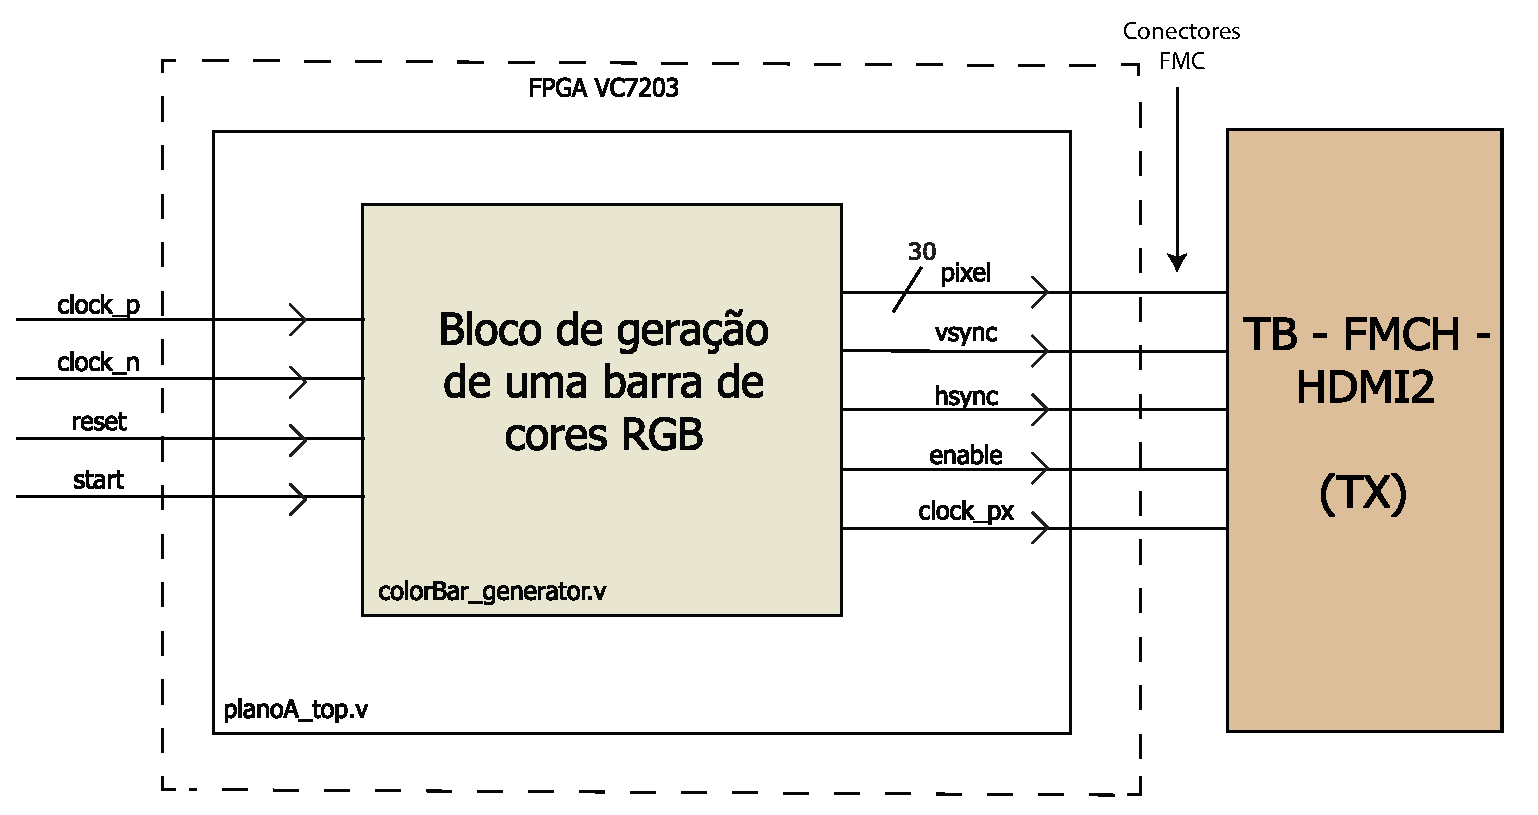
\includegraphics[width=1.0\textwidth]{planA}
		\caption{}
		\label{fig:planA}
	\end{center}
\end{figure}

\subsubsection{Transmissão de imagem entre dispositivos HDMI}

		\begin{figure}[h!]
	\begin{center}
		\leavevmode
		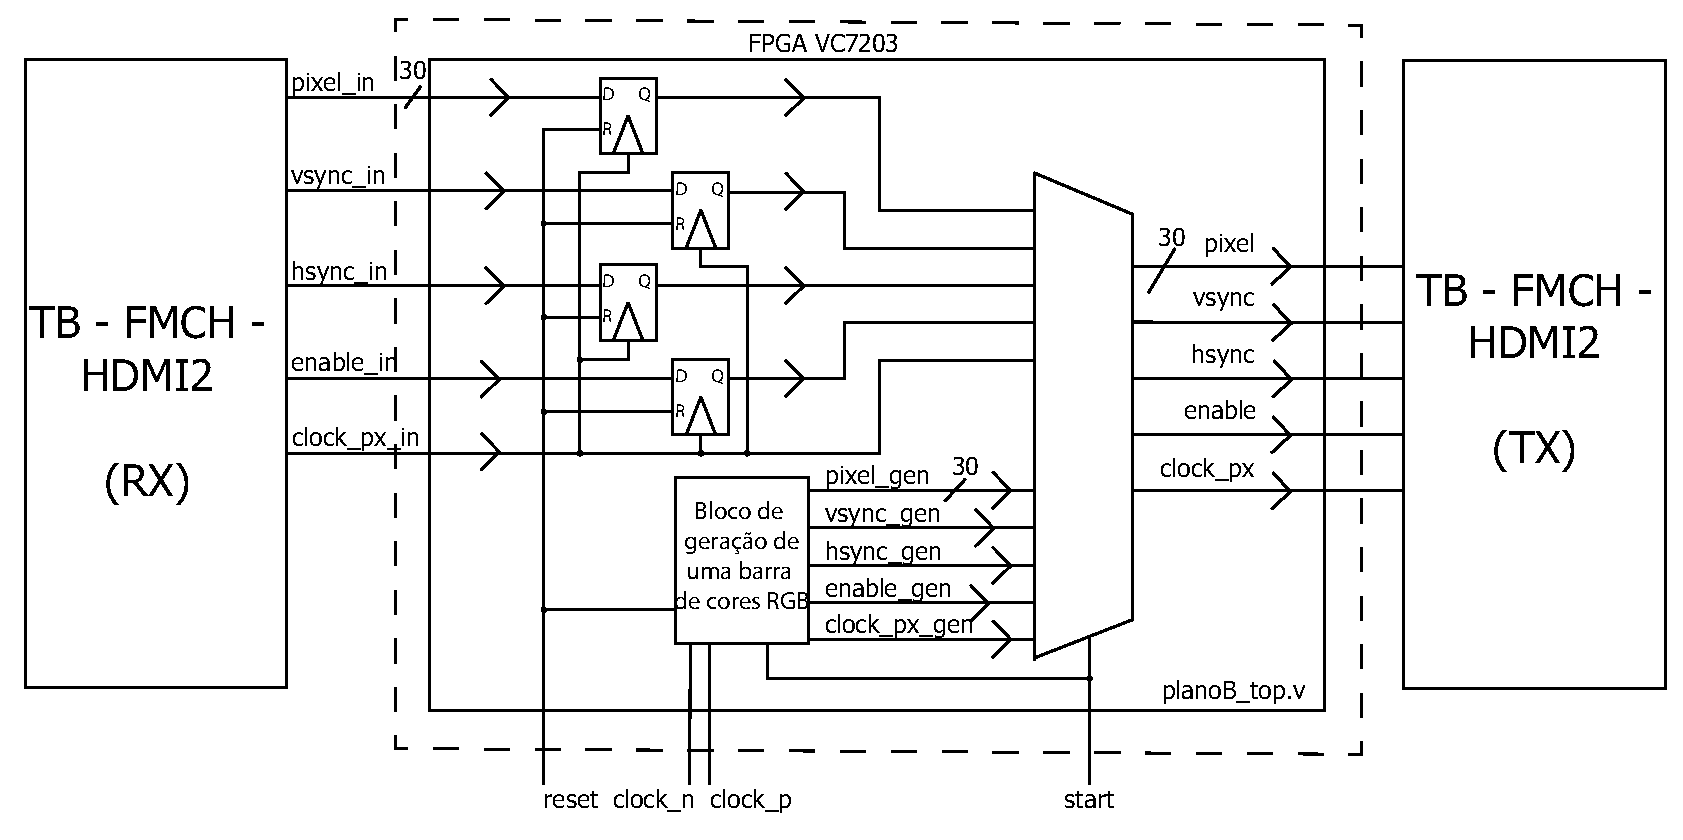
\includegraphics[width=1.0\textwidth]{planB1}
		\caption{}
		\label{fig:planb1}
	\end{center}
\end{figure}

\subsubsection{Transmissão de imagem e som entre dispositivos HDMI}